% Copyright (c)  2005-2010 EDF-EADS-PHIMECA.
% Permission is granted to copy, distribute and/or modify this document
% under the terms of the GNU Free Documentation License, Version 1.2
% or any later version published by the Free Software Foundation;
% with no Invariant Sections, no Front-Cover Texts, and no Back-Cover
% Texts.  A copy of the license is included in the section entitled "GNU
% Free Documentation License".
\renewcommand{\filename}{docUC_InputNoData_Copula}
\renewcommand{\filetitle}{UC : Creation of a copula and a composed copula}

% \HeaderNNIILevel
% \HeaderIILevel
\HeaderIIILevel








The objective of this Use Case is to manipulate copulas of Open TURNS.\\

A copula may be considered as the restriction to $[0,1]^n$ of a distribution with uniform 1D marginals on $[0,1]$ and this copula as copula. That's why an object of type {\itshape Copula} offers the same methods as an object of type {\itshape Distribution} (see U.C. \ref{manipulation_distribution} to have the list of the methods).\\

Details on copula may be found in the Reference Guide (\href{OpenTURNS_ReferenceGuide.pdf}{see file Reference Guide - Step B -- Copula}).\\

Details on each object may be found in the User Manual  (\href{OpenTURNS_UserManual_TUI.pdf}{see User Manual - Probabilistic modeling / Composed Distributions}).\\


\index{Copula!Composed copula}
\index{Copula!Clayton}
\index{Copula!Gumbel}
\index{Copula!Frank}
\index{Copula!Normal}
\index{Copula!Independent}
\index{Correlation!Correlation matrix of the Normal copula}
\index{Correlation!Spearman rank correlation matrix}


Open TURNS proposes some bidimensional copulas, listed in Table. \ref{ListCopulas}. One is elliptical : Normal copula, the others are archimedean : Frank, Clayton, Gumbel. The Independent one is both elliptical and archimedean.\\


Furthermore, Open TURNS is able to extract the copula $C$ from any $n$ dimensional distribution, thanks to the inverse of the Sklar theorem :
$$
C(u_1, \dots, u_n) = F(F_1^{-1}(u_1), \dots, F_n^{-1}(u_n))
$$
where $F$ is the cumulative density function of the distribution and $F_i$ its respective marginals. This copula is denoted \emph{Sklar Copula} within Open TURNS.\\


\newcommand\B{\rule[-2.4ex]{0pt}{0pt}}

\begin{table}[H]
  \begin{center}
    \begin{tabular}{|l|c|c|c|}
      \hline
      Name & Dimension & $C(u_1, \cdots, u_n)$ & Parameters\textspace\B\\
      \hline
      Independent & n& $\displaystyle \prod_{i=1}^{i=n} u_i$ & n \textspace\B\\
      \hline
      Normal & 2 &  $\displaystyle\int_{-\infty}^{\Phi^{-1}(u_1)}\int_{-\infty}^{\Phi^{-1}(u_2)}\frac{1}{2\pi\sqrt{1-\rho^2}}\exp\left(-\frac{s^2-2\rho st+t^2}{2(1-\rho^2)}\right)\,\Diff s\,\Diff t$ \mathspace\B & $\begin{array}{l}
        \mat{R} = \left(\begin{array}{cc}
            1 & \rho \\
            \rho & 1
          \end{array}
        \right)\\
        \rho \in [-1,1]
      \end{array}$\\
      \hline
      Normal & n & $\displaystyle\int_{-\infty}^{\Phi^{-1}(u_1)}\cdots \int_{-\infty}^{\Phi^{-1}(u_n)}\frac{1}{(2\pi)^{n/2} \sqrt{\det(\mat{R})}}\exp\left(-\frac{1}{2}\vect{x}^t \mat{R}^{-1} \vect{x} \right)\,\Diff \vect{x}$ & $\mat{R}$, SDP \textspace\B\\
      \hline
      % Student & 2 & $\displaystyle\int_{-\infty}^{T_{\nu}^{-1}(u_1)}\int_{-\infty}^{T_{\nu}^{-1}(u_2)}\frac{1}{2\pi\sqrt{1-\rho^2}}\left(1+\frac{s^2-2\rho st+t^2}{\nu(1-\rho^2)}\right)^{-(\nu+2)/2}\,\Diff s\,\Diff t$ & $\nu \in \mathbb{N}$ \mathspace\B\\
      % \hline
      Frank & 2 & $\displaystyle -\frac{1}{\theta}\log\left(1+\frac{(e^{-\theta u_1}-1)(e^{-\theta u_2}-1}{e^{-\theta}-1}\right)$ & $\theta \neq 0$\textspace\B\\
      \hline
      Clayton & 2 & $\displaystyle \left(u_1^{-\theta}+u_2^{-\theta}-1\right)^{-1/\theta}$ & $\theta \geq 0$\textspace\B\\
      \hline
      Gumbel & 2 & $\displaystyle \exp\left(-\left((-\log(u_1))^{\theta}+(-\log(u_2))^{\theta}\right)^{1/\theta}\right)$ & $\theta \geq 1$\textspace\B\\
      \hline
      Sklar & n & $\displaystyle F(F_1^{-1}(u_1), \dots, F_n^{-1}(u_n))$ & $-$\textspace\B\\
      \hline
    \end{tabular}
    \caption{Expressions of the copulas of Open TURNS.}
    \label{ListCopulas}
  \end{center}
\end{table}
\textspace\\


At last, Open TURNS enables to create some copula as the product of other copulas : if $C_1$ and $C_2$ are two copulas respectively of random vectors in  $\mathbb{R}^{n_1}$ and $\mathbb{R}^{n_2}$, we can create the copula of a random vector of $\mathbb{R}^{n_1+n_2}$, noted $C$ as follows :
$$
C(u_1, \cdots, u_n) = C_1(u_1, \cdots, u_{n_1}) C_2(u_{n_1+1}, \cdots, u_{n_1+n_2})
$$
It means that both subvectors $(u_1, \cdots, u_{n_1})$ and $(u_{n_1+1}, \cdots, u_{n_1+n_2})$ of $\mathbb{R}^{n_1}$ and $\mathbb{R}^{n_2}$ are independent.\\


\noindent%
\requirements{
  \begin{description}
  \item[$\bullet$] none
  \end{description}
}
{
  \begin{description}
  \item[$\bullet$] a Normal, Clayton, Gumbel, Frank, Independent and Min copulas : {\itshape normalCopula, claytonCopula, gumbelCopula, frankCopula, independentCopula, minCopula}
  \item[type:] NormalCopula, ClaytonCopula, GumbelCopula, FrankCopula, IndependentCopula, MinCopula
  \item[$\bullet$] a composed copula : {\itshape finalCopula}
  \item[type:] ComposedCopula
  \end{description}
}

\textspace\\
Python script for this UseCase :

\begin{lstlisting}

  # INDEPENDENT copula

  # Independent Copula parameterized by its dimension
  # For example, dimension = 3
  dim = 3
  independentCopula = IndependentCopula(dim)

  # Min Copula parameterized by its dimension
  # For example, dimension = 3
  dim = 3
  minCopula = MinCopula(dim)


  # NORMAL copula

  # Case 1 :  Normal Copula parameterized by its correlation matrix R

  # For example, dimension = 3 and R :
  dim = 3
  R =  CorrelationMatrix(dim)
  for i in range(dim-1) :
  R[i, i + 1] = 0.8

  # It is possible to define the correlation matrix through a map
  # and then use the function getCorrelationMatrixFromMap to convert
  # the map into a CorrelationMatrix
  # if input variables are noted X,Y and Z
  vars=['X','Y','Z']
  correlationMap={}
  correlationMap['X']={}
  correlationMap['X']['X']= 1.0
  correlationMap['X']['Y']= 0.8
  correlationMap['X']['Z']= 0.8
  correlationMap['Y']={}
  correlationMap['Y']['X']= 0.8
  correlationMap['Y']['Y']= 1.0
  correlationMap['Y']['Z']= 0.8
  correlationMap['Z']={}
  correlationMap['Z']['X']= 0.8
  correlationMap['Z']['Y']= 0.8
  correlationMap['Z']['Z']= 1.0
  R = getCorrelationMatrixFromMap(vars,correlationMap)


  # Create a normal copula from the correlation matrix R
  normalCopula = NormalCopula(R)
  normalCopula.setName("a normal copula")


  # Case 2 : Create a normal copula from the Spearman rank correlation matrix S

  # For example, dimension = 3 and S :
  dim = 3
  S = CorrelationMatrix(dim)
  for i in range(1,dim) :
  S[i, i - 1] = 0.25

  # Create the correlation matrix R of the  normal copula
  # from the Spearman correlation matrix S
  R = NormalCopula.GetCorrelationFromSpearmanCorrelation(S)

  # Create the normal copula from the R correlation matrix
  normalCopula = NormalCopula(R)
  normalCopula.setName("another normal copula")

  # Case 3 : Normal Copula parameterized by its dimension

  # Correlation matrix R is equal to identity
  dim = 3
  normalCopula = NormalCopula(dim)


  # CLAYTON copula

  # Only for dimension = 2
  # Clayton copula is parameterized by theta without restriction
  # For example, theta = -2.5
  theta = -2.5
  claytonCopula = ClaytonCopula(theta)


  # GUMBEL copula

  # Only for dimension = 2
  # Gumbel copula is parameterized by theta without restriction
  # For example, theta = 2.5
  theta = 2.5
  gumbelCopula = ClaytonCopula(theta)


  # FRANK copula

  # Only for dimension = 2
  # Frank copula is parameterized by theta without restriction
  # For example, theta = 9.2
  theta = 9.2
  frankCopula = FrankCopula(theta)

  # COMPOSED copula

  # For example, the GumbelCopula concatenated to a Clayton one
  # Create the collection of copulas
  copulaColl = CopulaCollection(2)
  copulaColl[0] = Copula(gumbelCopula)
  copulaColl[1] = Copula(claytonCopula)

  # Create the composed copula in R^4
  finalCopula = ComposedCopula(copulaColl)
\end{lstlisting}
\textspace\\

We draw in Figures \ref{IndependentCopulaIsoPDF} to \ref{FrankCopulaIsoPDF} the iso-curves of the PDF respectively of some copulas of type : Independent, Normal, Clayton, Gumbel, Frank.




\begin{figure}[H]
  \begin{minipage}{10cm}
    \begin{center}
      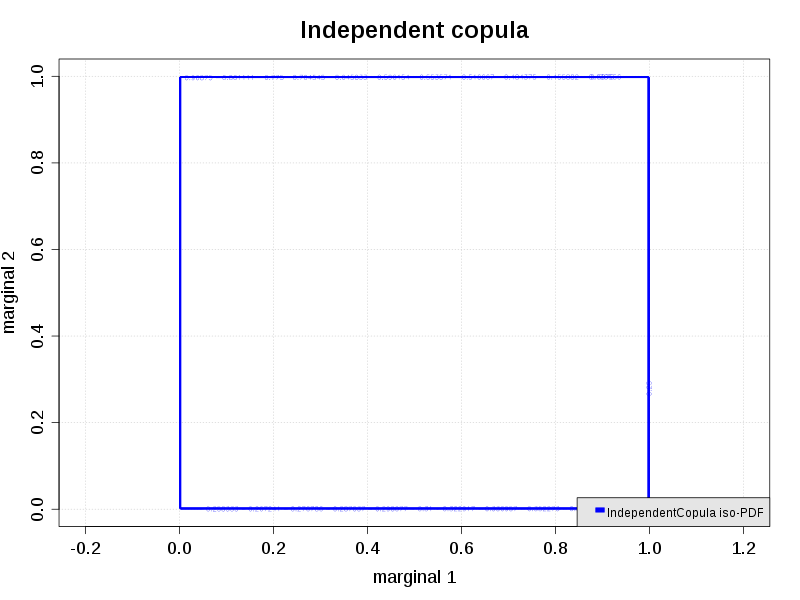
\includegraphics[width=7cm]{IndependentCopula.png}
      \caption{Iso-PDF of an independent copula.}
      \label{IndependentCopulaIsoPDF}
    \end{center}
  \end{minipage}
  \hfill
  \begin{minipage}{10cm}
    \begin{center}
      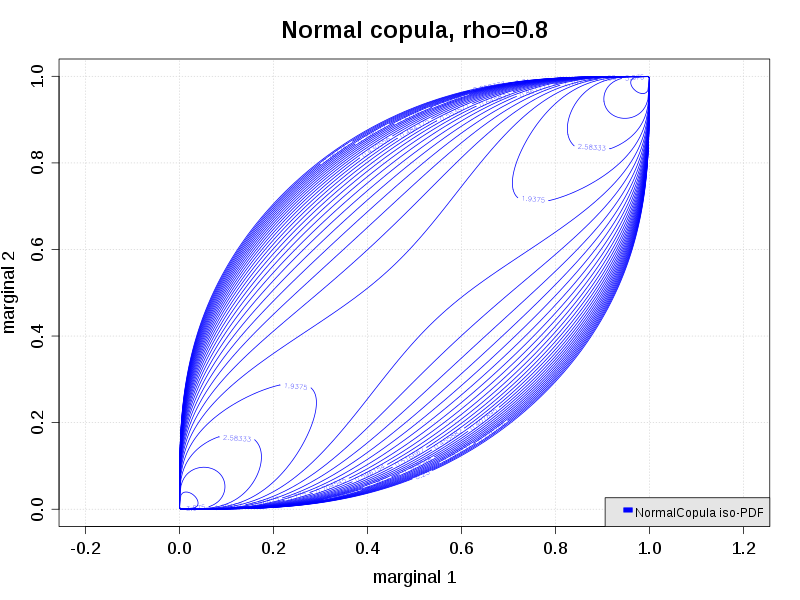
\includegraphics[width=7cm]{NormalCopula.png}
      \caption{Iso-PDF of a  Normal copula.}
      \label{NormalCopulaIsoPDF}
    \end{center}
  \end{minipage}
\end{figure}


\begin{figure}[H]
  \begin{minipage}{10cm}
    \begin{center}
      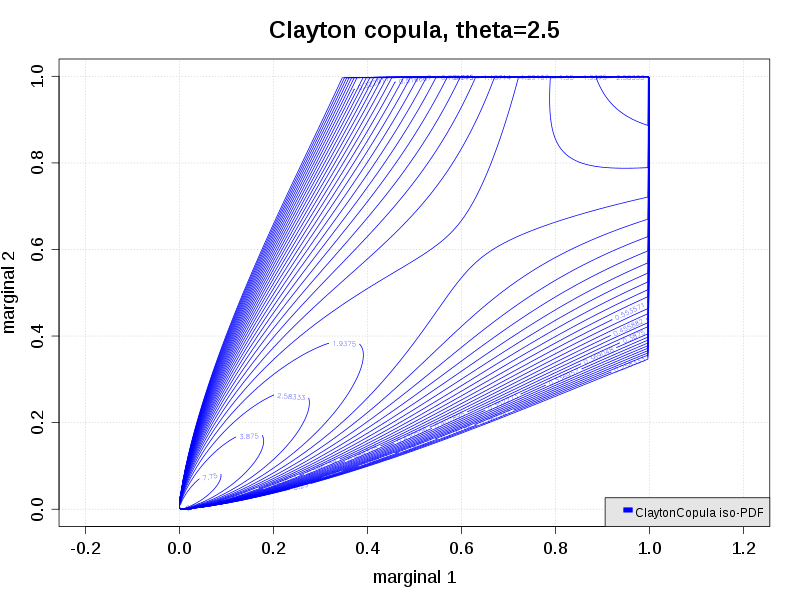
\includegraphics[width=7cm]{ClaytonCopula.png}
      \caption{Iso-PDF of a Clayton copula.}
      \label{ClaytonCopulaIsoPDF}
    \end{center}
  \end{minipage}
  \hfill
  \begin{minipage}{10cm}
    \begin{center}
      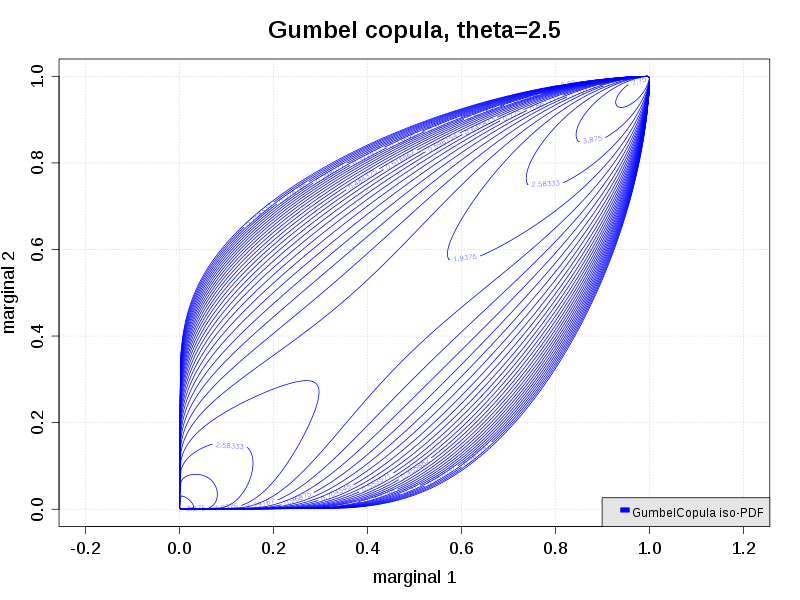
\includegraphics[width=7cm]{GumbelCopula.png}
      \caption{Iso-PDF of a Gumbel copula.}
      \label{GumbelCopulaIsoPDF}
    \end{center}
  \end{minipage}
\end{figure}


\begin{figure}[H]
  \begin{center}
    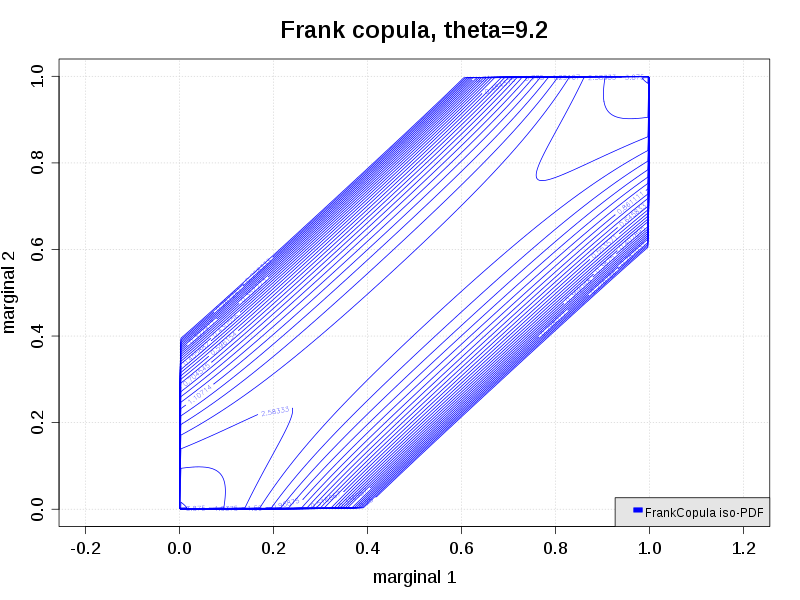
\includegraphics[width=7cm]{FrankCopula.png}
  \end{center}
  \caption{Iso-PDF of a Frank copula.}
  \label{FrankCopulaIsoPDF}
\end{figure}


